\section{Hardware dell'adapter board}
L'hardware utilizzato per condurre lo studio oggetto di questa tesi consiste in due piattaforme indossabili per effettuare misure fotopletismografiche. Ciascuna piattaforma si compone di una Adapter Board e una scheda ospitante un microcontrollore. L'\textit{Adapter Board} consiste in una PCB sulla quale sono montati il modulo PPG, un accelerometro ed un eventuale LDO per l'alimentazione dei componenti. Il microcontrollore viene utilizzato per l'acquisizione dei dati dai sensori e per il loro controllo. In particolare è stata utilizzata la board \textbf{STM32F4DISCOVERY}, prodotta da STMicroelectronics, in entrambi i casi, che ospita il micrcontrollore \textbf{STM32F407}.
La due piattaforme progettate si differenziano per l'Adapter Board, dal momento che sono stati utilizzati due differenti moduli PPG: il MAXM86161 e il MAX86916. Entrambi i sensori sono prodotti da Maxim Integrated.
\subsection{Adapter Board: MAXM86161}
\begin{figure}[h]
	\centering
	\includegraphics[width=0.8\linewidth]{ImageFiles/Hardware/diagramma_blocchi_MAXM}
	\caption{Diagramma a blocchi della piattaforma con sensore MAXM86161.}
	\label{fig:diagramma_blocchi_MAXM}
\end{figure}
L'Adapter Board è la scheda che monta il sensore PPG utilizzato per fare le acquisizioni che, vengono fatte con la board STM32F4DISCOVERY. I due sottosistemi utilizzano il protocollo I\ap{2}C per comunicare. 
Come riportato in figura \Fig~\ref{fig:diagramma_blocchi_MAXM}, la scheda contiene solamente il sensore PPG e un accelerometro triassiale. Grazie al numero ridotto di componenti è stato possibile ottenere una scheda dalle dimensioni molto piccole (12,4 x 4,6 mm).
\begin{figure}[h]
	\centering
	\includegraphics[width=0.8\linewidth]{ImageFiles/Hardware/MAXM86161_Layout}
	\caption{MAXM86161 magari evidenziare i led e fotodiodo}
	\label{fig:MAXM86161_Layout}
\end{figure}
\paragraph{Sensore PPG} Il sensore PPG utilizzato è il MAXM86161 \Fig~\ref{fig:MAXM86161_Layout}, prodotto da Maxim Integrated, descritto precedentemente come stato dell'arte. Si tratta quindi di un circuito integrato, a basso consumo, per acquisizioni di dati ottici. Il sensore integra 3 LED (rosso, infrarosse e verde), un fotodiodo e un regolatore di tensione lineare(LDO), che viene utilizzato per fornire l'alimentazione ai LED. Il MAXM86161 necessita di una singola tensione di alimentazione che deve essere compresa tra i 3.0V e 5.5V. Le dimensioni di questo modulo sono estremamente ridotte (2.9mm x 4.3mm x 1.4mm), che lo rendono molto flessibile nelle modalità di utilizzo e sopratutto adatto per sistemi di misura indossabili.

\paragraph{Accelerometro} Insieme alle acquisizioni del sensore PPG vengono integrate anche delle misure accelero-metriche. L'accelerometro utilizzato è \textbf{LIS2DH12} \cite{STMicroelectronicsLIS2DH12} prodotto da STMicroelectronics. Si tratta di un accelerometro triassiale a basso consumo e dalle piccole dimensioni (2 x 2 mm). Questo sensore viene utilizzato per migliorare la qualità delle acquisizioni fotopletismografiche quando il soggetto è in movimento, fornendo un'informazione sull'entità di quest'ultimo, e quindi del disturbo che si introduce nella misura. Il LIS2DH12 richiede una tensione di alimentazione compresa tra i 1.71V e i 3.6V, con un consumo di corrente pari a \SI{185}{\micro\ampere}.

\paragraph{Progetto PCB}

\subsection{Adapter Board: MAX86916}
Questa \textit{Adapter Board} invece contiene tre circuiti integrati che sono: il sensore PPG, un regolatore di tensione (LDO) e un accelerometro.
\begin{figure}[h]
	\centering
	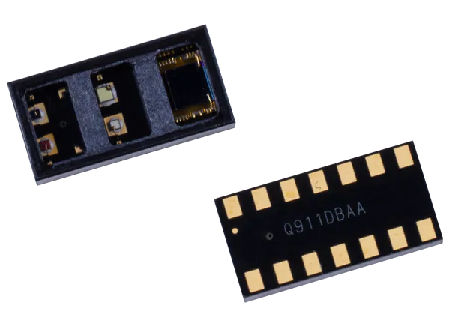
\includegraphics[width=0.6\linewidth]{ImageFiles/Hardware/MAX86916_Layout}
	\caption{MAX86916 magari mettere in evidenza led e foto diodo}
	\label{fig:MAX86916_Layout}
\end{figure}

\paragraph{Sensore PPG} Il sensore PPG utilizzato è il MAX86916, prodotto da Maxim Integrated, descritto precedentemente come stato dell'arte.

\paragraph{LDO} \todo{Parliamo dei 3 LDO che abbiamo valutato? si parlerei di tutti e tre o almeno 2 mettendo in evidenza magari una tabella con le differenze}

\paragraph{Accelerometro}\todo{ut supra} L'accelerometro utilizzato è sempre \textbf{LIS2DH12} prodotto da STMicroelectronics.

\subsection{Microcontrollore: STM32F4DISCOVERY}\todo{farei una descrizione con alcune nozione sui componenti}
\todo{inserire immagine della board}